\documentclass[11pt,spanish,a4paper,hidelinks]{book}
\usepackage[utf8]{inputenc}
\usepackage{graphicx}
\graphicspath{{graficos/}}
\usepackage{tikz}
\usetikzlibrary{calc}
\pgfdeclarelayer{background}
\pgfdeclarelayer{foreground}
\pgfsetlayers{background,main,foreground}
\usepackage{fontspec}
\setmainfont{Times New Roman} 
\usepackage{amsmath}
\usepackage{amsfonts}
\usepackage{ifthen}
\usepackage{tabularx}
%%%%%%%%%%%%%%%%%%%%%%%%%%%%%%%%%%%%%%%%%%%%%%%%%%%%%%%%%%
\usepackage{colortbl}
\definecolor{Lightgray}{RGB}{235,235,235}
%%%%%%%%%%%%%%%%%%%%%%%%%%%%%%%%%%%%%%%%%%%%%%%%%%%%%%%%%%
\setlength{\parskip}{6pt}
%%%%%%%%%%%%%%%%%%%%%%%%%%%%%%%%%%%%%%%%%%%%%%%%%%%%%%%%%%
\setcounter{tocdepth}{4}
\setcounter{secnumdepth}{4}
%%%%%%%%%%%%%%%%%%%%%%%%%%%%%%%%%%%%%%%%%%%%%%%%%%%%%%%%%%
\usepackage[
inner	=	3.0cm, % Margen interior
outer	=	3.0cm, % Margen exterior
top	=	2.5cm, % Margen superior
bottom=	2.5cm, % Margen inferior
includeheadfoot, % Incluye cabecera y pie de página en los márgenes
]{geometry}
\renewcommand{\baselinestretch}{1.0}
\usepackage{xcolor}
\usepackage{sectsty}
%%%%%%%%%%%%%%%%%%%%%%%%%%%%%%%%%%%%%%%%%%%%%%%%%%%%%%%%
\definecolor{azul}{rgb}{0.1,0.2,0.4}
\chapterfont{\color{azul}}  % sets colour of chapters
\sectionfont{\color{azul}}  % sets colour of sections
\subsectionfont{\color{azul}}  % sets colour of sections
\subsubsectionfont{\color{azul}}  % sets colour of sections
%%%%%%%%%%%%%%%%%%%%%%%%%%%%%%%%%%%%%%%%%%%%%%%%%%%%%%%%
\usepackage[style=numeric,sorting=none]{biblatex}
\addbibresource{referencias.bib}
%%%%%%%%%%%%%%%%%%%%%%%%%%%%%%%%%%%%%%%%%%%%%%%%%%%%%%%%
\usepackage{booktabs}
\usepackage{threeparttable}
%%%%%%%%%%%%%%%%%%%%%%%%%%%%%%%%%%%%%%%%%%%%%%%%%%%%%%%%
\usepackage{tocloft}
\cftpagenumbersoff{part}
%%%%%%%%%%%%%%%%%%%%%%%%%%%%%%%%%%%%%%%%%%%%%%%%%%%%%%%
\usepackage[nonumberlist,automake]{glossaries}
% Generate the glossary
\makeglossaries
%%%%%%%%%%%%%%%%%%%%%%%%%%%%%%%%%%%%%%%%%%%%%%%%%%%%%%%%
\defbibheading{firstlevel}[]{%
	\chapter*{#1}
	\addcontentsline{toc}{chapter}{#1}}
%%%%%%%%%%%%%%%%%%%%%%%%%%%%%%%%%%%%%%%%%%%%%%%%%%%%%%%%
\usepackage[spanish]{babel}
%%%%%%%%%%%%%%%%%%%%%%%%%%%%%%%%%%%%%%%%%%%%%%%%%%%%%%%%
\usepackage{hyperref}
%%%%%%%%%%%%%%%%%%%%%%%%%%%%%%%%%%%%%%%%%%%%%%%%%%%%%%%%
\usepackage{fancyhdr}% http://ctan.org/pkg/fancyhdr
\pagestyle{fancy}% Change page style to fancy
%\fancyhf{}% Clear header/footer
%\fancyhead[C]{Header}
%%%%%%%  %%%%%%%%%%%  %%%%%%  %%%%%%%%%%%%%%%%%%%%%%%%
%Opción 1) capítulo y sección en cada página
%\fancyhead[LE,RO]{\footnotesize\color{azul}\rightmark}
%\fancyhead[LO,RE]{\footnotesize\color{azul}\leftmark}
%Opción 2) capítulo y sección se alternan
\fancyhead[LE]{\footnotesize\color{azul}\leftmark}
\fancyhead[RO]{\footnotesize\color{azul}\rightmark}
\fancyhead[LO,RE]{}
%%%%%%  %%%%%%%%%%  %%%%%%%%%%  %%%%%%%%%%%%%%%%%%%%%%%%

\fancyfoot[C]{\footnotesize\color{azul} \thepage}% \fancyfoot[R]{\thepage}
\renewcommand{\headrulewidth}{0.4pt}% Default \headrulewidth is 0.4pt
\renewcommand{\footrulewidth}{0.4pt}% Default \footrulewidth is 0pt
\makeatletter
\renewcommand{\headrule}{\setlength\@tempdima{\headrulewidth}
	\textcolor{azul}{\hrule\@height\@tempdima\@width\headwidth}
	\vskip -2\@tempdima}
\makeatother
\renewcommand{\footrule}{\hbox to\headwidth{\color{azul}\leaders\hrule height \footrulewidth\hfill}}

% Redefine the plain page style
\fancypagestyle{plain}{%
	\fancyhf{}%
	\fancyfoot[C]{\footnotesize\color{azul} \thepage}%
	\renewcommand{\headrulewidth}{0pt}% Line at the header invisible
	\renewcommand{\footrulewidth}{0.4pt}% Line at the footer visible
}
%%%Acercar texto y línea en cabecera
\makeatletter
\def\headrule{{
		\if@fancyplain\let\headrulewidth\plainheadrulewidth\fi
		\vskip0pt% change here
		\color{azul}\hrule\@height\headrulewidth\@width\headwidth   
		\vskip-\headrulewidth%
}}
%%%%%%%%%%%%%%%%%%%%%%%%%%%%%%%%%%%%%%%%%%%%%%%%%%%%%%%%
%Part reinicia la numeración de capítulos
\makeatletter
\@addtoreset{chapter}{part}
\makeatother
%%%%%%%%%%%%%%%%%%%%%%%%%%%%%%%%%%%%%%%%%%%%%%%%%%%%%%%%
%Part sin numeración de página
\makeatletter
\renewcommand\part{%
	\if@openright
	\cleardoublepage
	\else
	\clearpage
	\fi
	\thispagestyle{empty}%   % Original »plain« replaced by »emptyx
	\if@twocolumn
	\onecolumn
	\@tempswatrue
	\else
	\@tempswafalse
	\fi
	\null\vfil
	\secdef\@part\@spart}
\makeatother
%%%%%%%%%%%%%%%%%%%%%%%%%%%%%%%%%%%%%%%%%%%%%%%%%%%%%%%%
%Pie de figura en negrita
\usepackage[labelfont=bf]{caption}%Solo Figura XX
%\usepackage[font=bf]{caption}%Todo el pie de figura
%%%%%%%%%%%%%%%%%%%%%%%%%%%%%%%%%%%%%%%%%%%%%%%%%%%%%%%%
%DESCOMENTAR para tener numeración de figuras y tablas 
%continua en todo el documento
%\renewcommand\thefigure{\arabic{figure}}
%\renewcommand\thetable{\arabic{table}}
%\renewcommand\theequation{\arabic{equation}}
%\setcounter{figure}{0}

%\usepackage{chngcntr}
%\counterwithout{figure}{chapter}
%\counterwithout{table}{chapter}
%counterwithout{equation}{chapter}

%%%%%%%%%%%%%%%%%%%%%%%%%%%%%%%%%%%%%%%%%%%%%%%%%%%%%%%%
%DESCOMENTAR PARA ELIMINAR EL INDENTADO INICIAL DE LOS PÁRRAFOS
%\setlength{\parindent}{0pt}

\raggedbottom
%%%%%%%%%%%%%%%%%%%%%%%%%%%%%%%%%%%%%%%%%%%%%%%%%%%%%%%%%%%%%%%%%%%%%%%
%                   COMPILAR CON XELATEX
%%%%%%%%%%%%%%%%%%%%%%%%%%%%%%%%%%%%%%%%%%%%%%%%%%%%%%%%%%%%%%%%%%%%%%%
\newcommand{\titulo}{TÍTULO DEL TFM (EN MAYÚSCULAS)}
\newcommand{\tutorA}{Nombre y apellidos del tutor}
\newcommand{\tutorB}{Nombre y apellidos del cotutor (en su caso)} % En su caso. En blanco si no hay.
\newcommand{\tutorE}{Nombre y apellidos del tutor en la empresa (en su caso)} %En su caso. En blanco si no hay.
\newcommand{\curso}{2019-20} %(curso que proceda)
\newcommand{\autor}{Autor del Trabajo Final de Máster}
\newcommand{\fecha}{Septiembre  de  2019} %mes y año            
%%%%%%%%%%%%%%%%%%%%%%%%%%%%%%%%%%%%%%%%%%%%%%%%%%%%%%%%%%%%%%%%%%%%%%
%%%%%%%%%%%%%%%%%%%%%%%%%%%%%%%%%%%%%%%%%%%%%%%%%%%%%%%%%%%%%%%%%%%%%%%
%Si alguna página de la tabla de contenidos tiene encabezado o pie de
%página, probar a añadir estas líneas tras el \chapter{} de uno de los 
%capítulos/anexos que aparezcan en esa página
%\addtocontents{toc}{\protect\thispagestyle{empty}}
%\addtocontents{toc}{\protect\pagestyle{empty}}
%%%%%%%%%%%%%%%%%%%%%%%%%%%%%%%%%%%%%%%%%%%%%%%%%%%%%%%%%%%%%%%%%%%%%%%
%%%%%%%%%%%%%%%%%%%%%%%%%%%%%%%%%%%%%%%%%%%%%%%%%%%%%%%%%%%%%%%%%%%%%%%
\begin{document}
	\renewcommand{\listtablename}{Índice de tablas} 
	\renewcommand{\tablename}{Tabla} 
	%\headrulecolor{azul}
	\thispagestyle{empty}
	%%%%%%%%%%%%%%%%%%%%%%%%%%%%%%%%%%%%%%%%%%%%%%%%%%%%%%%%%%%%%%%%%%%%%%%%%%
%%%%%%%%%%%%%%%%%%%%%%%%%%%%%%%%%%%%%%%%%%%%%%%%%%%%%%%%%%%%%%%%%%%%%%%%%%

\begin{tikzpicture}[overlay,remember picture]
	%\node at (current page.center) {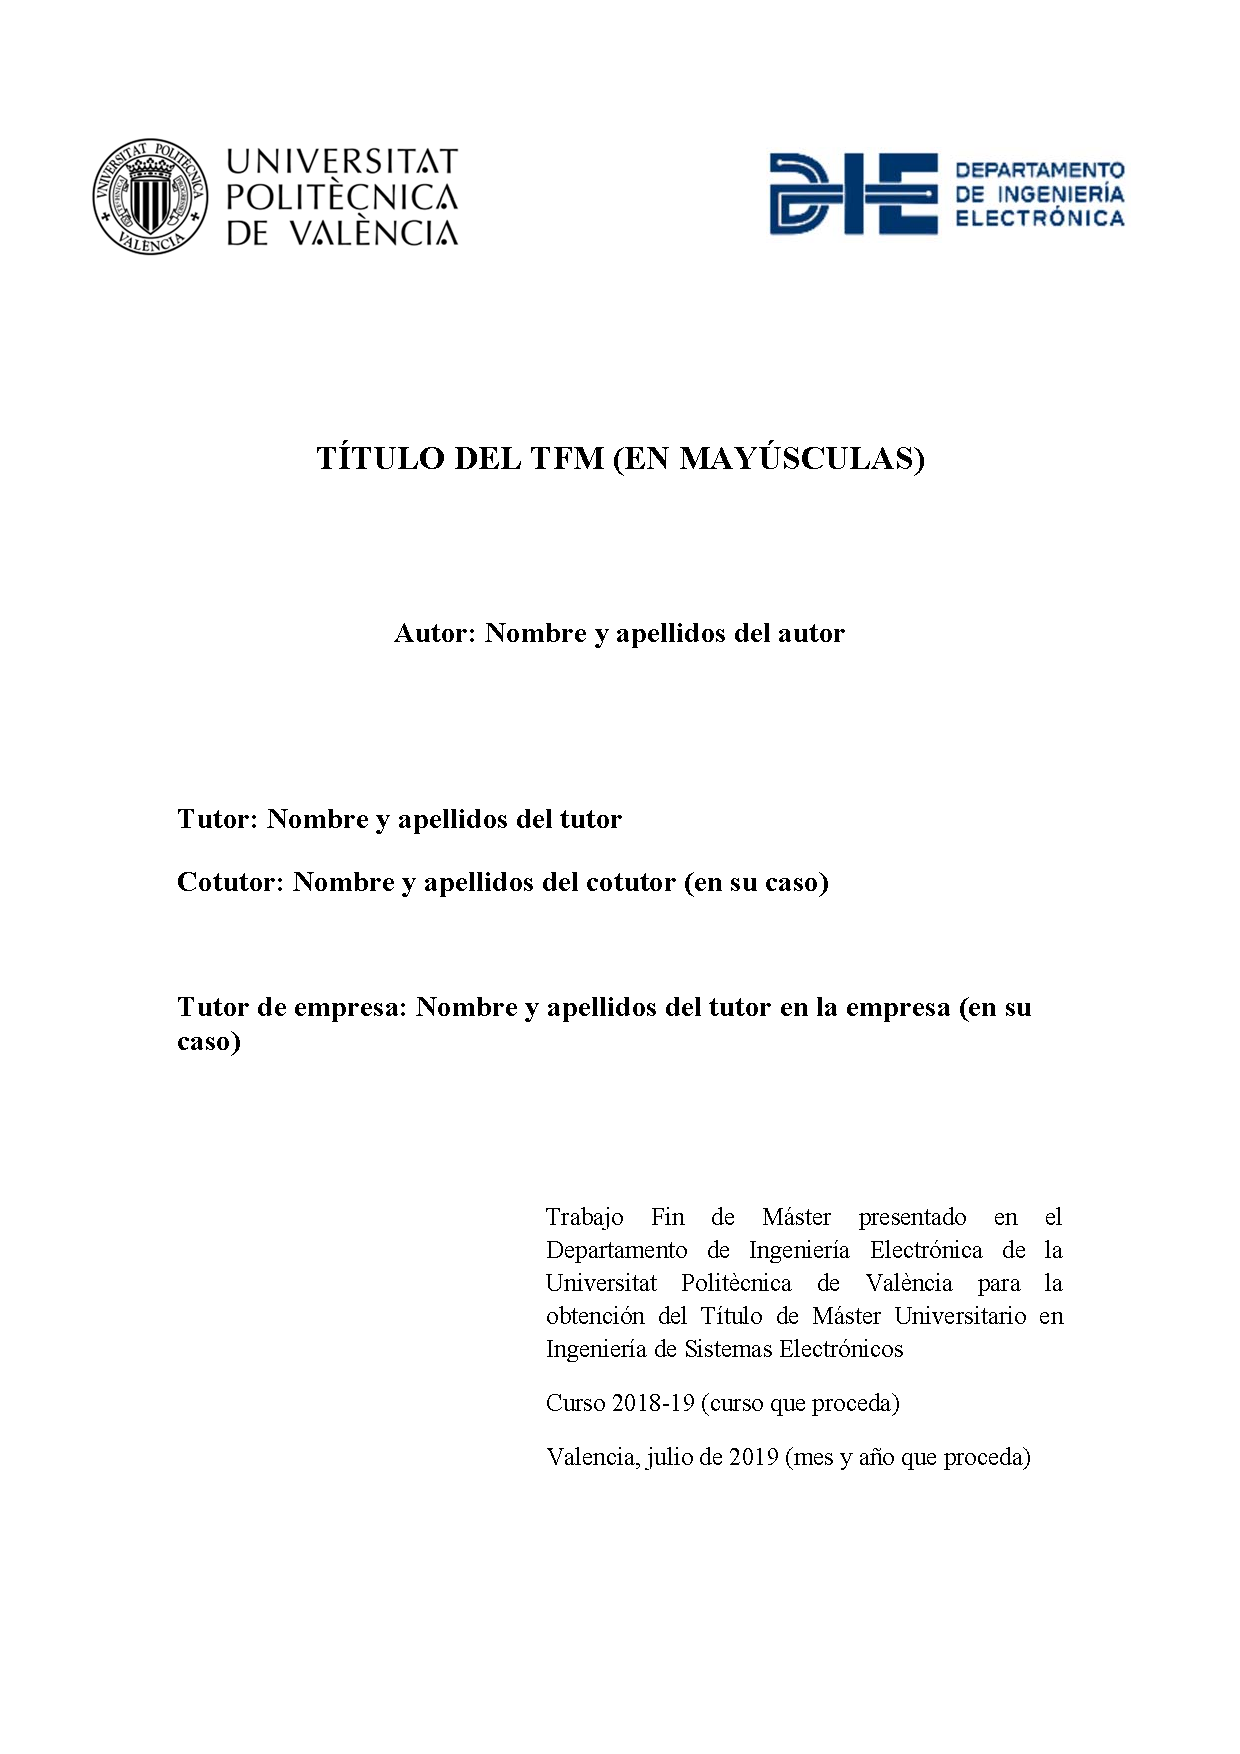
\includegraphics[page=1]{Plantilla_Memoria_TFM_PDF-2018.pdf}};
	\node at ($(current page.north)+(-5.8cm,-3.3cm)$) {
\includegraphics[scale=0.72]{marca_UPV_principal_negro.pdf}};
	\node at ($(current page.north)+(5.55cm,-3.3cm)$) {
\includegraphics[trim=0mm 0mm 0mm 0,clip,width=0.4\textwidth]{logo_die.pdf}};
	\node[anchor=center] at ($(current page.center)!0.48!(current page.north)+(0cm,0)$) (titulo){\begin{minipage}{\textwidth}\begin{center}\LARGE\textbf{\uppercase{\titulo}}\end{center}\end{minipage}};
	
	\node[anchor=north west] at  ($(current page.center)+(-1.45cm,-5.475cm)$) (){\parbox{0.585\textwidth}{%
			\rmfamily
			\tolerance=1%
			\emergencystretch=\maxdimen%
			\hyphenpenalty=10000%
			\hbadness=10000%
			\large Trabajo   Fin   de   Máster   presentado   en   el Departamento  de  Ingeniería  Electrónica  de  la Universitat   Politècnica   de   València   para   la obtención  del  Título  de  Máster  Universitario  en Ingeniería de Sistemas Electrónicos\newline
			\ \\
			Curso \curso\\ 
			\ \\
			Valencia, \fecha}};
	\node[anchor=west] at ($(current page.west)+(2.85cm,0.9cm)$) (tutor){\Large\bfseries Tutor: \tutorA};
	\node[anchor=west] at ($(current page.west)+(2.85cm,-0.1cm)$) {\Large\bfseries \ifthenelse{\equal{\tutorB}{}}{}{Cotutor: \tutorB}};
	\node[anchor=west] at ($(current page.west)+(2.85cm,-2.25cm)$) {\Large\bfseries \ifthenelse{\equal{\tutorE}{}}{}{Tutor de Empresa: \tutorE}};
	\node[coordinate] at ($(titulo.south)!(tutor.north)!(titulo.south)$) (tutornorte){}; %altura de tutor pero centrado
	\node at ($(titulo.south)!0.49!(tutornorte)$) (){\begin{minipage}{\textwidth}\begin{center}\Large\textbf{Autor: \autor}\end{center}\end{minipage}};
\end{tikzpicture}

	\newpage
	\thispagestyle{empty}\ \\
	\newpage
	\thispagestyle{empty}
	
	\section*{Resumen}
	\noindent La memoria comienza con un breve resumen de entre 
	100 y 300
	palabras, escrito en castellano,
	valenciano e inglés. No numerar estas páginas.
	Resum
	
	
	\section*{Resum}
	\noindent La memoria del TFG comença amb un breu resum d’entre 
	100 i 300
	paraules, escrit en castellà, valencià i anglès. Aquestes pàgines van sense numerar.
	
	
	\section*{Abstract}
	\noindent The memory of the TFG begins with a short abstract from 
	100 and 300
	words, writen in Spanish, Valencian and English. These pages are not numbered.
	
	\newpage
	\thispagestyle{empty}
	\ \\
	\vfill\begin{flushright}
		A mis padres.
	\end{flushright}\vfill\vfill
	
	\newpage
	\thispagestyle{empty}
	\ \\
	\addtocontents{toc}{\protect\thispagestyle{empty}}
	\addtocontents{toc}{\protect\pagestyle{empty}}
	\tableofcontents\newpage\thispagestyle{empty}
	\addtocontents{lof}{\protect\thispagestyle{empty}}
	\addtocontents{lof}{\protect\pagestyle{empty}}
	\listoffigures\thispagestyle{empty}\newpage\thispagestyle{empty}
	\addtocontents{lot}{\protect\thispagestyle{empty}}
	\addtocontents{lot}{\protect\pagestyle{empty}}
	\listoftables\thispagestyle{empty}\newpage\thispagestyle{empty}
	\newpage\thispagestyle{empty}
	
\newglossaryentry{utc}{name=UTC, description={Coordinated Universal Time}}
\newglossaryentry{adt}{name=ADT, description={Atlantic Daylight Time}}
\newglossaryentry{est}{name=EST, description={Eastern Standard Time}}
\newglossaryentry{lna}{name=LNA, description={Amplificador de Bajo Ruido (Low Noise Amplifier)}}

%\gls{utc} is 3 hours behind \gls{adt} and 10 hours ahead of \gls{est}.

\printglossary[title={\color{black}Listado de siglas empleadas}, toctitle=Listado de siglas]
	\thispagestyle{empty}
	\setcounter{page}{-2}
	\newpage
	\addtocontents{toc}{\protect\thispagestyle{empty}}
	\part{Memoria}
	
	\chapter{Introducción}
\noindent En la introducción se situará el contexto del trabajo realizado, identificando claramente el problema que se plantea y soluciones para el mismo que se hayan propuesto previamente. 

No hay máximo ni mínimo en cuanto a la extensión de la memoria del TFM, pero se debe buscar un equilibrio entre síntesis y completitud. 50 a 80 páginas más anexos suele ser suficiente.

\noindent La estructura de la memoria del TFM deberá reflejar, al menos, los siguientes contenidos:
\begin{itemize}
	\item Portada con título del TFM, nombres del autor y tutores, logotipo de la UPV y el Departamento de Ingeniería Electrónica, fecha (mes, año) y curso académico en el que realizó la defensa del TFM.
	\item  Índice de contenidos.
	\item  Introducción, en la que se situará el contexto del trabajo realizado, identificando claramente el problema que se plantea y soluciones para el mismo que se hayan propuesto previamente.
	\item  Descripción de la solución o las soluciones estudiadas.
	\item  Presentación de resultados tanto analíticos como de simulación y experimentales.
	\item  Conclusiones, en las que se hará un balance crítico de los resultados alcanzados.
	\item  Propuesta de actividades a desarrollar en el futuro, incluyendo, si fuera el caso, la línea de trabajo sobre la que se realizaría una futura tesis doctoral.
	\item  Referencias.
	\item  Anexos (si procede). En este apartado se pueden añadir esquemas electrónicos, detalles de cálculos largos, desarrollos matemáticos largos, hojas de datos que se considere imprescindibles, etc.
\end{itemize}


\chapter{Formato de la Memoria}
\section{Idioma}
\noindent La memoria se podrá escribir en castellano, valenciano o inglés.
\section{Tipo de letra y tamaño de página}
\noindent La memoria podrá estar realizada en cualquier formato que se pueda convertir a PDF (Word, \TeX,...) y se usará letra Book Antiqua, Times New Roman, Calibri o Arial de tamaño 11 puntos. El tamaño de página será A4 con márgenes superior e inferior 2,5 cm, márgenes izquierdo y derecho 3 cm.
\section{Estructura}
\subsection{Párrafos}
\noindent La memoria se escribirá en párrafos justificados a izquierda y derecha. Se usará un interlineado sencillo con una separación entre párrafos mínima de 6 puntos.
\subsection{Capítulos, Secciones y Subsecciones}
\noindent Los capítulos irán numerados y se dividirán en secciones y subsecciones con la numeración correspondiente.  
\section{Figuras, tablas y ecuaciones}
\noindent Las tablas y las figuras tendrán su correspondiente numeración en el pie de las mismas, que dará una breve descripción y citará a la referencia de la que procede, si es el caso. Las ecuaciones también irán numeradas. La numeración puede dar cuenta del capítulo en que se encuentra la tabla, figura o ecuación, si el alto número así lo aconseja. Las figuras pueden contener subfiguras, por ejemplo la Figura~\mbox{\ref{fig:subfigs}(a)} y \mbox{\ref{fig:subfigs}(b)}. La Figura~\ref{fig:PLL2} es otro ejemplo.

Las Tablas~\ref{tab:ejemplo} y \ref{tab:tablagris2} son ejemplos de tabla.

\begin{figure}
	\centering
	\includegraphics[page=6,trim=3.5cm 10.75cm 3.5cm 2.5cm 0,clip]{Plantilla_Memoria_TFM_PDF-2018.pdf}
	\caption{Ejemplo de figura con dos subfiguras. (a) descripción de la figura superior. (b) descripción de la figura
		inferior. }
	\label{fig:subfigs}
\end{figure}
\begin{figure}
	\centering
	\resizebox{\textwidth}{!}{\begin{tikzpicture}[ultra thick,black,opacity=1]
			\tikzset{bloque/.style={draw=black, rectangle,draw=blue, fill=lightgray!20, rounded corners,minimum width=2cm,minimum height=1cm,ultra thick}}
			\node[bloque] at (0,0) (PC){\shortstack{Phase\\comparator}};
			\node[bloque] at (3,0) (LF){\shortstack{Loop\\filter}};
			\node[bloque] at (6,0) (VCO){\shortstack{VCO}};
			\node[circle,fill=black,draw=black,inner sep=0.5mm] at ($(VCO.east)+(0.5cm,0)$) (nodo){};
			\draw[latex-] (PC.west) -- +(-1,0) node[pos=1,anchor=east](){$V_i$};
			\draw[-latex] (VCO.east) -- +(1,0) node[pos=1,anchor=west](){$V_o$};
			\draw[-latex] (nodo) -- +(0,-1)  -| (PC);
			\draw[-latex] (PC) -- (LF);
			\draw[-latex] (LF) -- (VCO);
	\end{tikzpicture}}
	\caption{Ejemplo de figura}
	\label{fig:PLL2}
\end{figure}

\begin{table}[]
	\centering
	\begin{tabular}{@{} *5l @{}}    \toprule
		\emph{name} & \emph{foo} &&&  \\\midrule
		Models    & A  & B  & C  & D  \\ 
		Model $X$ & X1 & X2 & X3 & X4\\ 
		Model $Y$ & Y1 & Y2 & Y3 & Y4\\\bottomrule
		\hline
	\end{tabular}
	\caption{Tabla ejemplo}
	\label{tab:ejemplo}
\end{table}

\begin{table}[]
	\centering
	\begin{tikzpicture}
		\node[inner sep=0pt,outer sep=0pt] (tbl) {
			\begin{tabularx}{.75\textwidth}{ p{0.15 \textwidth}  p{0.10 \textwidth} p{0.10 \textwidth} p{0.10 \textwidth} p{0.15 \textwidth}  }
				\toprule
				& Small  &  Medium &  Large & Shape fraction \\
				\midrule
				Compact    & 10\% &  44\% & 7\% & 61\% \\ 
				Flat       & 4\%  &  10\% & 4\% & 18\% \\ 
				Elongated  & 5\%  &  12\% & 4\% & 21\% \\ 
				\midrule 
				Size fraction  & 19\% & 66\% & 15\% & 100\% \\
				\bottomrule
		\end{tabularx}};
		\begin{pgfonlayer}{background}
			\draw[top color=lightgray,bottom color=lightgray!10!white,
			draw=none] ($(tbl.north west)+(0,0)$)
			rectangle ($(tbl.north east)+(0,-1.9em)$);
			\draw[fill=white,draw=none] ($(tbl.south west)
			+(0,0)$) rectangle ($(tbl.north east)+(0,-1.9em)$);
		\end{pgfonlayer}
	\end{tikzpicture}
	\caption{Otra tabla}
	\label{tab:tablagris2}
\end{table}


Ejemplos de ecuaciones (\ref{eq:muise1}, \ref{eq:muise2} y \ref{eq:muise3}):
\begin{equation}
	\label{eq:muise1}
	\textrm{PF}=\frac{I_{1\_\textrm{RMS}}}{I_{\textrm{RMS}}}{\cdot}\cos\varphi_1
\end{equation}

\begin{equation}
	\label{eq:muise2}
	(1+x)^n=1+\frac{n x}{1!}+\frac{n (n-1)x^2}{2!}+\ldots
\end{equation}

\begin{align}
	\mathbb{X}[z]&=\sum_{n=0}^{N-1}x[n]{\cdot}z^{-n}
	=\sum_{n=0}^{\infty} a^{-n}{\cdot}z^{-n}=\nonumber\\
	\label{eq:muise3}
	&=\frac{1}{1-(a{\cdot}z)^{-1}}=\frac{z}{z{-}a^{-1}}
\end{align}

\section{Referencias bibliográficas}

\noindent Se debe incluir las referencias bibliográficas o de internet de las fuentes consultadas y/o
utilizadas en la memoria. Estas referencias deberán ser correctamente citadas en el texto, dando
siempre el debido reconocimiento a las fuentes de información. Se pueden listar en el apartado
de referencias con diferentes estilos.
Por ejemplo, numéricamente entre corchetes como se muestra en la bibliografía.

Citando una referencia \cite{Smith1997}, otra \cite{Orfanidis1996} y otra \cite{Wyndrum1965}. Y otra más \cite{Dai2010}.

\section{Lista de siglas empleadas}

Para que las siglas empleadas aparezcan en el listado de siglas, al principio del documento, hay que definirlas en ``siglas.tex'' y también usarlas en el documento con el comando \verb+\gls+: \gls{utc}, \gls{lna} y \gls{adt} se están usando de esa manera. %Directrices TFM MUISE
	
	%%%%%%%%%%%%%%%%%%%%%%%%%%%%%%%%%%%%%%%%%%%%%%%%%%%%%%%%%%%%%%%%%%%%%%%
	%%%%%%%%%%%%%%%%%%%%%%%%%%%%%%%%%%%%%%%%%%%%%%%%%%%%%%%%%%%%%%%%%%%%%%%
	\printbibliography[heading=firstlevel,title=Bibliografía]
	%\addcontentsline{toc}{chapter}{Bibliografía}
	\label{sec:biblio}
	\newpage\thispagestyle{empty}
	%%%%%%%%%%%%%%%%%%%%%%%%%%%%%%%%%%%%%%%%%%%%%%%%%%%%%%%%%%%%%%%%%%%%%%%
	%%%%%%%%%%%%%%%%%%%%%%%%%%%%%%%%%%%%%%%%%%%%%%%%%%%%%%%%%%%%%%%%%%%%%%%
	\part{Anexos}
	\def\thechapter{\Alph{chapter}}
	\makeatletter
	\renewcommand{\@chapapp}{Apéndice}
	\makeatother
	\chapter{Listados adicionales}
	
	Ejemplo.
\end{document}

